\section{Separate modern extension: saved exploratory evidence}\label{app:modern}
The following results reproduce the separately authorized October 20, 2026 extension specified in the dated modern-analysis amendment. They are not new analyses for this manuscript and are not pooled with the annual 1900--2010 estimates. Prior modern outcome exposure remains undocumented, so the extension is exploratory rather than an untouched confirmatory holdout. This distinction holds even though the saved claim models were frozen and their historical predictions were reproduced before application.\evidence{N1--N2}

\subsection{Intake, maturity, and frozen claim models}
The intake has 91,118 retained candidates. Removing 19 default-kept verification exceptions leaves 91,099 primary inputs; 33,071 no-prediction records are separately excluded from inputs. The source exports retain their original bytes and row addresses. Of the primary candidate inputs, 32,604 lack supported scope, topic, direction, or horizon; 1,138 are unmatured; and 471 have reference gaps. The evaluated set therefore contains 56,886 mature, supported claims from 23,775 articles. Missing outcomes are not interpolated.

The modern claim models use unchanged historical fitted parameters. The deterministic outcome rules retain a three-month maturity allowance as of October 20, 2026. The saved reference run records failed refresh attempts and uses preserved snapshots, including production, CPI, and unemployment through June 2026. This is a dated evaluation, not a claim that the manuscript refreshed all economic series to its preparation date.

\begin{table}[t]
\caption{Modern claim-correctness prediction: frozen baseline and secondary arms}\label{tab:modern}
\centering\small
\begin{tabularx}{\linewidth}{Xrrrr}
\toprule
Model & AUC & Brier & Log loss & Accuracy\\
\midrule
Metadata logistic & .662 & .1983 & .5861 & .6987\\
Metadata + history logistic & .654 & .1936 & .5789 & .7223\\
Frozen GRU, baseline & .738 & .1770 & .5347 & .7539\\
GRU + political separation & .692 & .1826 & .5503 & .7618\\
GRU + forecast disagreement & .712 & .1819 & .5479 & .7388\\
GRU + both measures & .749 & .1742 & .5259 & .7610\\
Historical 8-unit challenger & .723 & .1775 & .5792 & .7743\\
\bottomrule
\end{tabularx}
\note{56,886 common claims, equal article weights. Positive correctness prevalence is .2868. The historical challenger is disclosed without promotion. Accuracy uses a .5 decision threshold; a classifier always predicting incorrect would attain .7132 accuracy from the evaluated prevalence, so accuracy alone is not a strong skill diagnostic. Source: N1.}
\end{table}

The primary GRU's Brier improvement over metadata-plus-history logistic is 0.0165, with a paired five-year block interval of $[-0.0092,0.0376]$. The baseline GRU minus the both-measures GRU yields an improvement of 0.0028 for the added inputs, with interval $[-0.0058,0.0191]$. These intervals do not establish the primary gains. The simpler metadata-only comparison has an interval favoring the GRU, but it is a weaker information-set comparator and does not override the primary comparison. There are four occupied blocks with 17,784, 18,017, 21,072, and only 13 claims, respectively. The nominal block count overstates the amount of balanced temporal replication.

Political separation and forecast disagreement measure different constructs. The former uses prior House rollcalls, averaging the absolute Democratic--Republican difference in actual yes-vote shares over a twelve-month window ending two months before the origin. The latter averages $4p_+p_-$ over three completed print months for business claims, with documented coverage rules. It measures opposing directional camps, not newspaper political ideology. Both are lagged; retrospective database curation remains different from archived real-time releases. Neither predictive association identifies a causal effect of polarization.\evidence{P3}

\subsection{Calibration and topic failure}
Discrimination varies substantially. The primary GRU's modern AUC is 0.906 for prices (6,750 claims), 0.788 for markets (9,234), 0.767 for general business (33,509), and 0.306 for employment (7,393). Employment Brier is 0.2707. AUC below 0.5 indicates that the saved ranking is reversed relative to the correctness label in that subgroup; it does not establish that employment forecasts themselves have an accuracy of 30.6\%, nor license post hoc reversal of the model as a validated remedy.

\begin{figure}[t]
\centering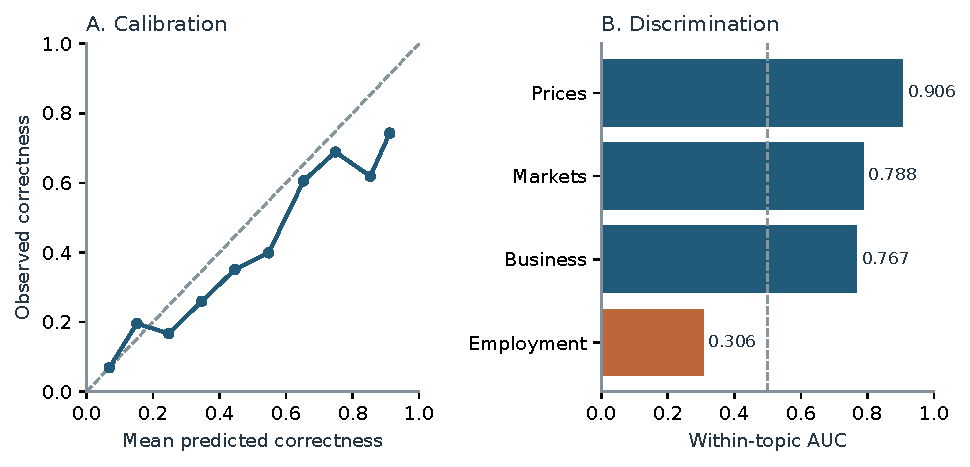
\includegraphics[width=\linewidth]{modern_diagnostics.pdf}
\caption{Saved modern diagnostics for the primary frozen GRU. Panel A uses the saved article-weighted calibration bins; the diagonal is perfect calibration. Panel B displays topic-specific AUC, with the .5 reference marked. Pooled performance conceals substantial employment failure and overconfidence in several probability bins. Source: N1.}\label{fig:modern}
\end{figure}

Calibration also limits interpretation. In the .8--.9 bin, mean predicted correctness is .853 but observed correctness is .619 across 2,168 claims. In the highest bin, the corresponding values are .912 and .743 across 474 claims. These are saved weighted bin means with unweighted claim counts, not independent-bin inference. They demonstrate why an AUC of .738 should not be translated into well-calibrated probabilities. No evaluation-set recalibration is introduced in this manuscript.

\subsection{Separate monthly downturn models}
The downturn exercise uses separately fitted monthly logistic models. Its recession-onset target is any transition from nonrecession to recession in months $t$ through $t+11$; an already ongoing recession is not a new onset. Its production-decline target compares industrial production at $t+11$ with $t-1$. The main production target is any decline, with a greater-than-2\% sensitivity. These are distinct from claim correctness and from the historical six-month, three-class macro target.

Five candidates per target comprise an expanding, Laplace-smoothed event base rate and four ridge logistic variants: press only, press plus political separation, press plus forecast disagreement, and press plus both. Annual January refits admit only mature prior outcomes, using a 24-month allowance for recession dating and three months for production. Candidate selection uses pre-2011 rolling Brier results and remains fixed for modern evaluation. Revised assessment outcomes and reconstructed vote data mean this is not a complete vintage-real-time exercise.\evidence{N2}

\begin{table}[t]
\caption{Modern downturn evaluation against the event base rate}\label{tab:downturn}
\centering\small
\begin{tabularx}{\linewidth}{Xrrr}
\toprule
Target and selected model & Origins & Brier & Base-rate Brier\\
\midrule
Recession onset; press + both & 154 & .0696 & .0832\\
Any production decline; press + forecast disagreement & 175 & .2272 & .2570\\
\bottomrule
\end{tabularx}
\note{Selections were made using pre-2011 performance. Five-year paired intervals for base-rate minus selected-model Brier are [$-.0100$,$.0246$] for onset and [$-.0312$,$.0692$] for production decline. Each uses three occupied blocks and 2,000 draws. The downturn study supplies no matched modern macro-only benchmark. Source: N2.}
\end{table}

The 154 evaluated recession origins contain twelve positive monthly labels but only one distinct onset, March 2020. Those labels arise from overlapping forecast windows rather than twelve independent recessions. The production evaluation contains 175 origins and 69 positive labels. The selected improvements have intervals crossing zero, and the greater-than-2\% production sensitivity performs worse than its base-rate comparator. These results cannot establish stable superiority over macroeconomic forecasting models, since a matched modern macro-only comparison is absent.

\subsection{Dated forecast illustration}
The latest complete newspaper inputs end in August 2026. At the September 2026 origin, the preselected models assign 6.88\% to a recession onset and 28.00\% to any industrial-production decline over September 2026--August 2027. The recession base-rate comparator is 17.36\%, and all candidate onset estimates range from 6.88\% to 27.03\%. The selected production estimate is nearly identical to its 28.01\% base rate. Recent feature support comprises 56 articles from five papers across three observed print months.

These figures demonstrate how the fitted procedure produces a dated forecast. They are not an October-origin forecast, a mature observed outcome, or evidence of a successful downturn prediction. A prospective record should preserve this origin, input cutoff, target, and model selection before the evaluation window ends. Updating inputs or selecting a different candidate later would create a new forecast rather than validate this one retroactively.

